\subsection{Interrelación Asignatura Curso Académico - Alumno Curso Académico}

   \begin{description}
      \item[Definición] En esta interrelación se deja constancia de que un
      alumno matriculado durante un curso académico está matriculado de un
      determinado de un número indeterminado de asignaturas, las cuales
      pertenecen a un determinado curso académico.

      \item[Características] La interrelación presenta las siguientes
                             características:

         \begin{itemize}
            \item \textbf{Nombre:} ACA-AlCA
            \item \textbf{Tipo de la interrelación:} Fuerte.
            \item \textbf{Cardinalidad de la interrelación:} N:M
            \item \textbf{Número de atributos:} 1, nota.
         \end{itemize}

      \item[Diagrama] La figura \ref{diagramaACA-AlCA} muestra el diagrama de la
                      interrelación.

       \item \begin{figure}[!ht]
            \begin{center}
            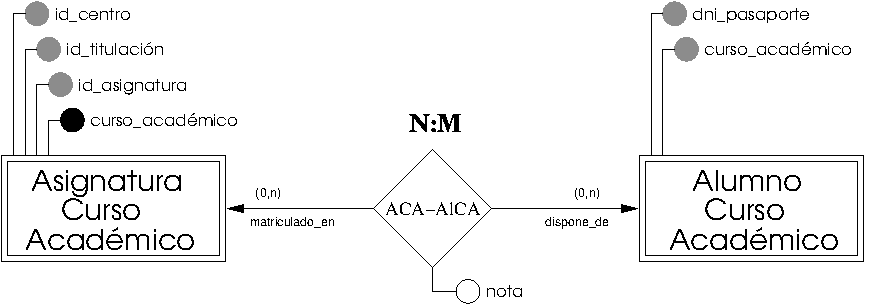
\includegraphics[]{07.Modelo_Entidad-Interrelacion/7.3.Analisis_Interrelaciones/diagramas/ACA-AlCA.pdf}
            \caption{Diagrama de la interrelación ACA-AlCA.}
            \label{diagramaACA-AlCA}
            \end{center}
         \end{figure}

      \item[Descripción de los atributos]

      \item \begin{description}
               \item[Nota] Establece la calificación obtenida por un alumno en
               una asignatura durante un curso académico.
             \end{description}

      \item[Ejemplo práctico del tipo de interrelación]

      \item \begin{center}
            \begin{tabular}{ | c | c | c | }
            \hline
            \multicolumn{2}{ | c | }{\textbf{Tipo de interrelación ACA-AlCA}} \\
            \hline
            \textbf{Asignatura Curso Académico} & \textbf{Alumno Curso Académico} & Atributos\\
            \hline
            id\_centro+id\_titulación+id\_asignatura+curso\_académico & dni\_pasaporte+curso\_académico & Nota \\
            \hline
            153172008 & 01234567A2008 & 7.5 \\
            \hline
            \end{tabular}
         \end{center}
   \end{description}
